\chapter{Выполнение задания}

\section{Реализуемый алгоритм}
Сортировка слиянием

\section{Выбор языка программирования}
Для выполнения домашнего задания был выбран язык \texttt{C++}.

\section{Код программы}

В листинге \ref{lst:merge} приведена реализация алгоритма сортировки слиянием.

\lstinputlisting[label=lst:merge, caption=Реализация алгоритма сортировки слиянием, firstline=9,lastline=60]{../code/main.cpp}

\section{Модели программ}

На рисунках \ref{fg:mg}--\ref{fg:ii_2} представлены модели графовых управлений.

\subsection{Граф управления программы}

\begin{figure}[h]
	\centering
	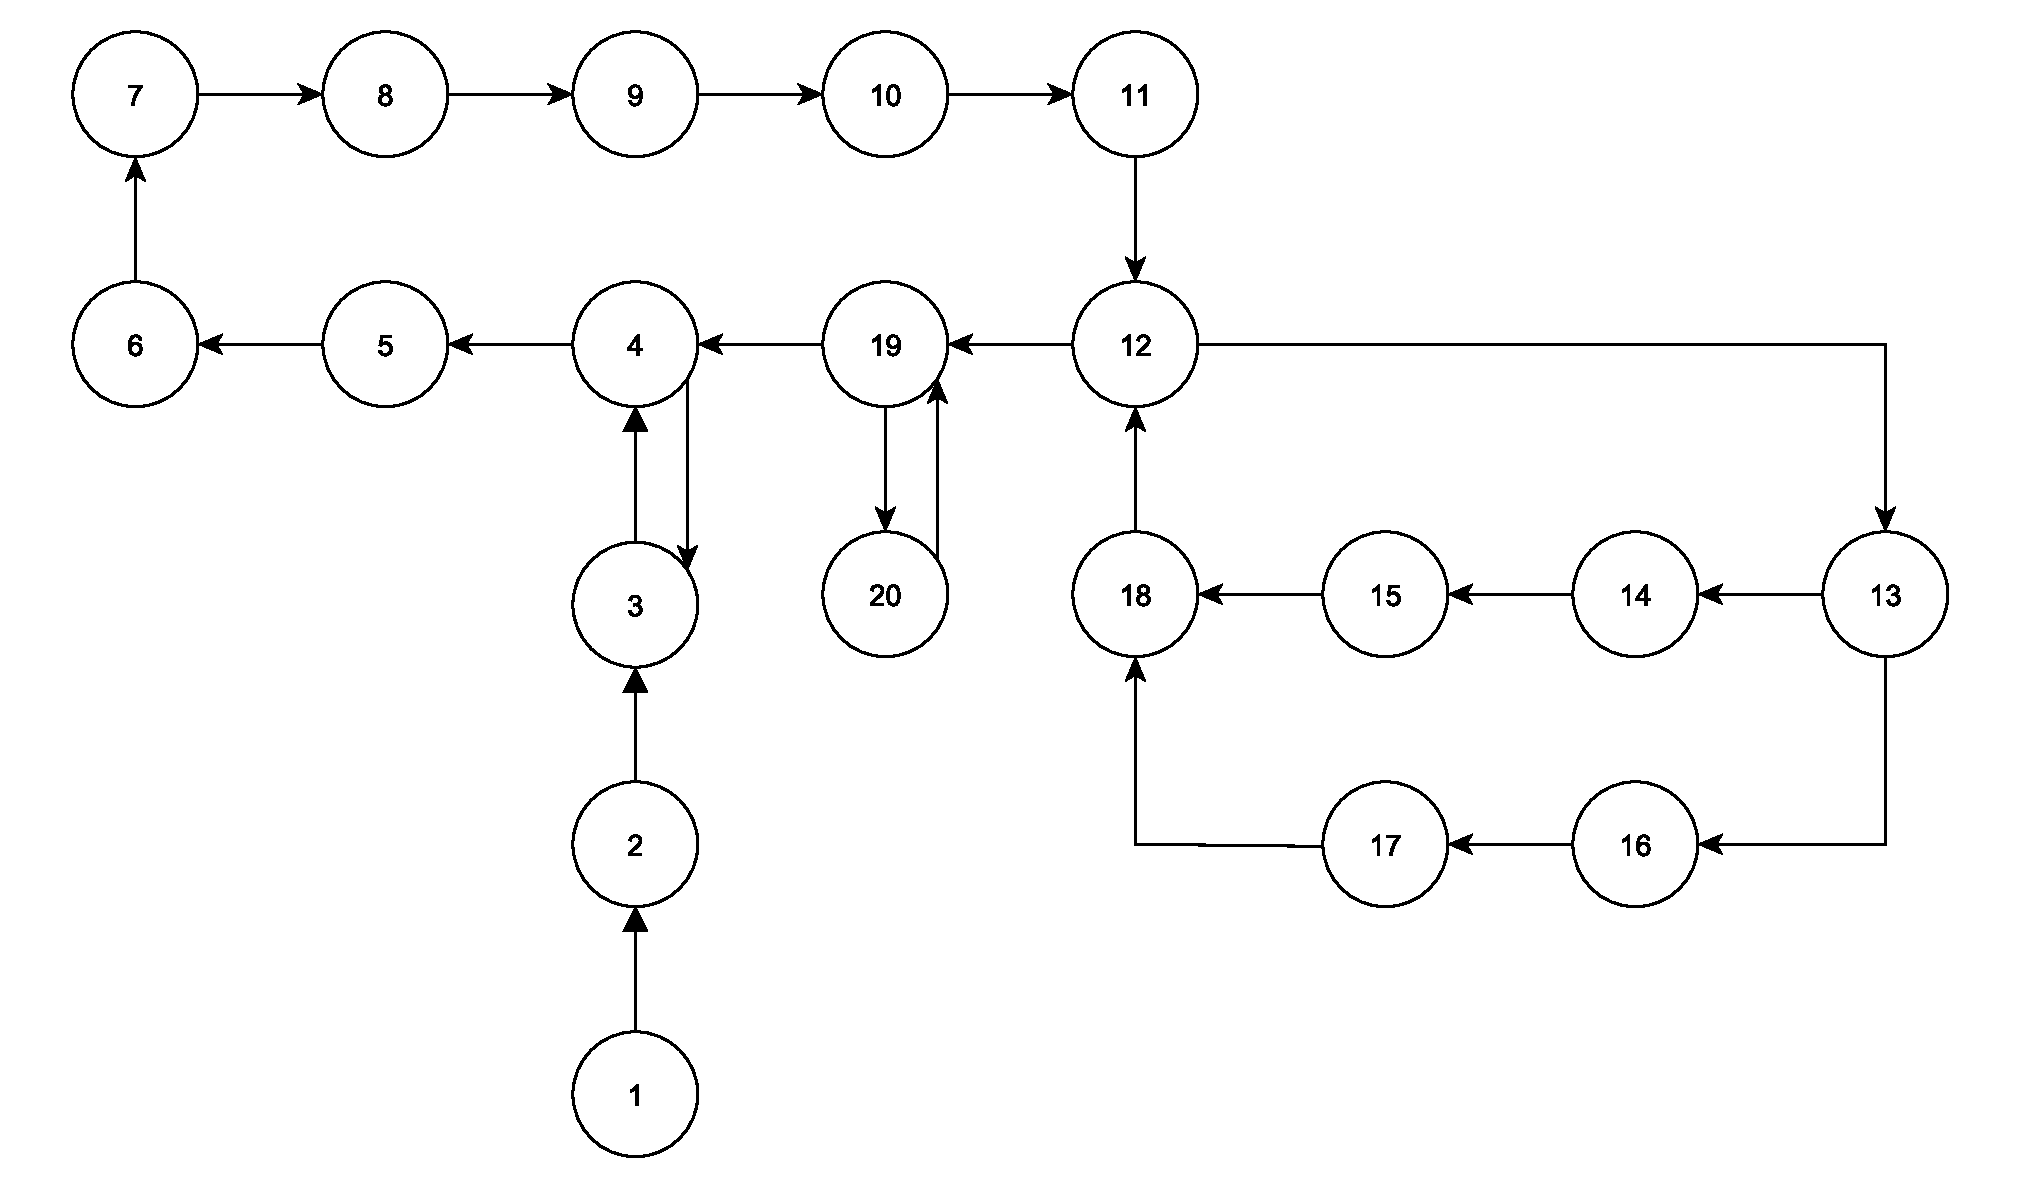
\includegraphics[height=0.4\textheight]{img/граф_управления.pdf}
	\caption{Граф управления}
	\label{fg:mg}
\end{figure}

\clearpage

\subsection{Информационный граф программы}

\begin{figure}[h]
	\centering
	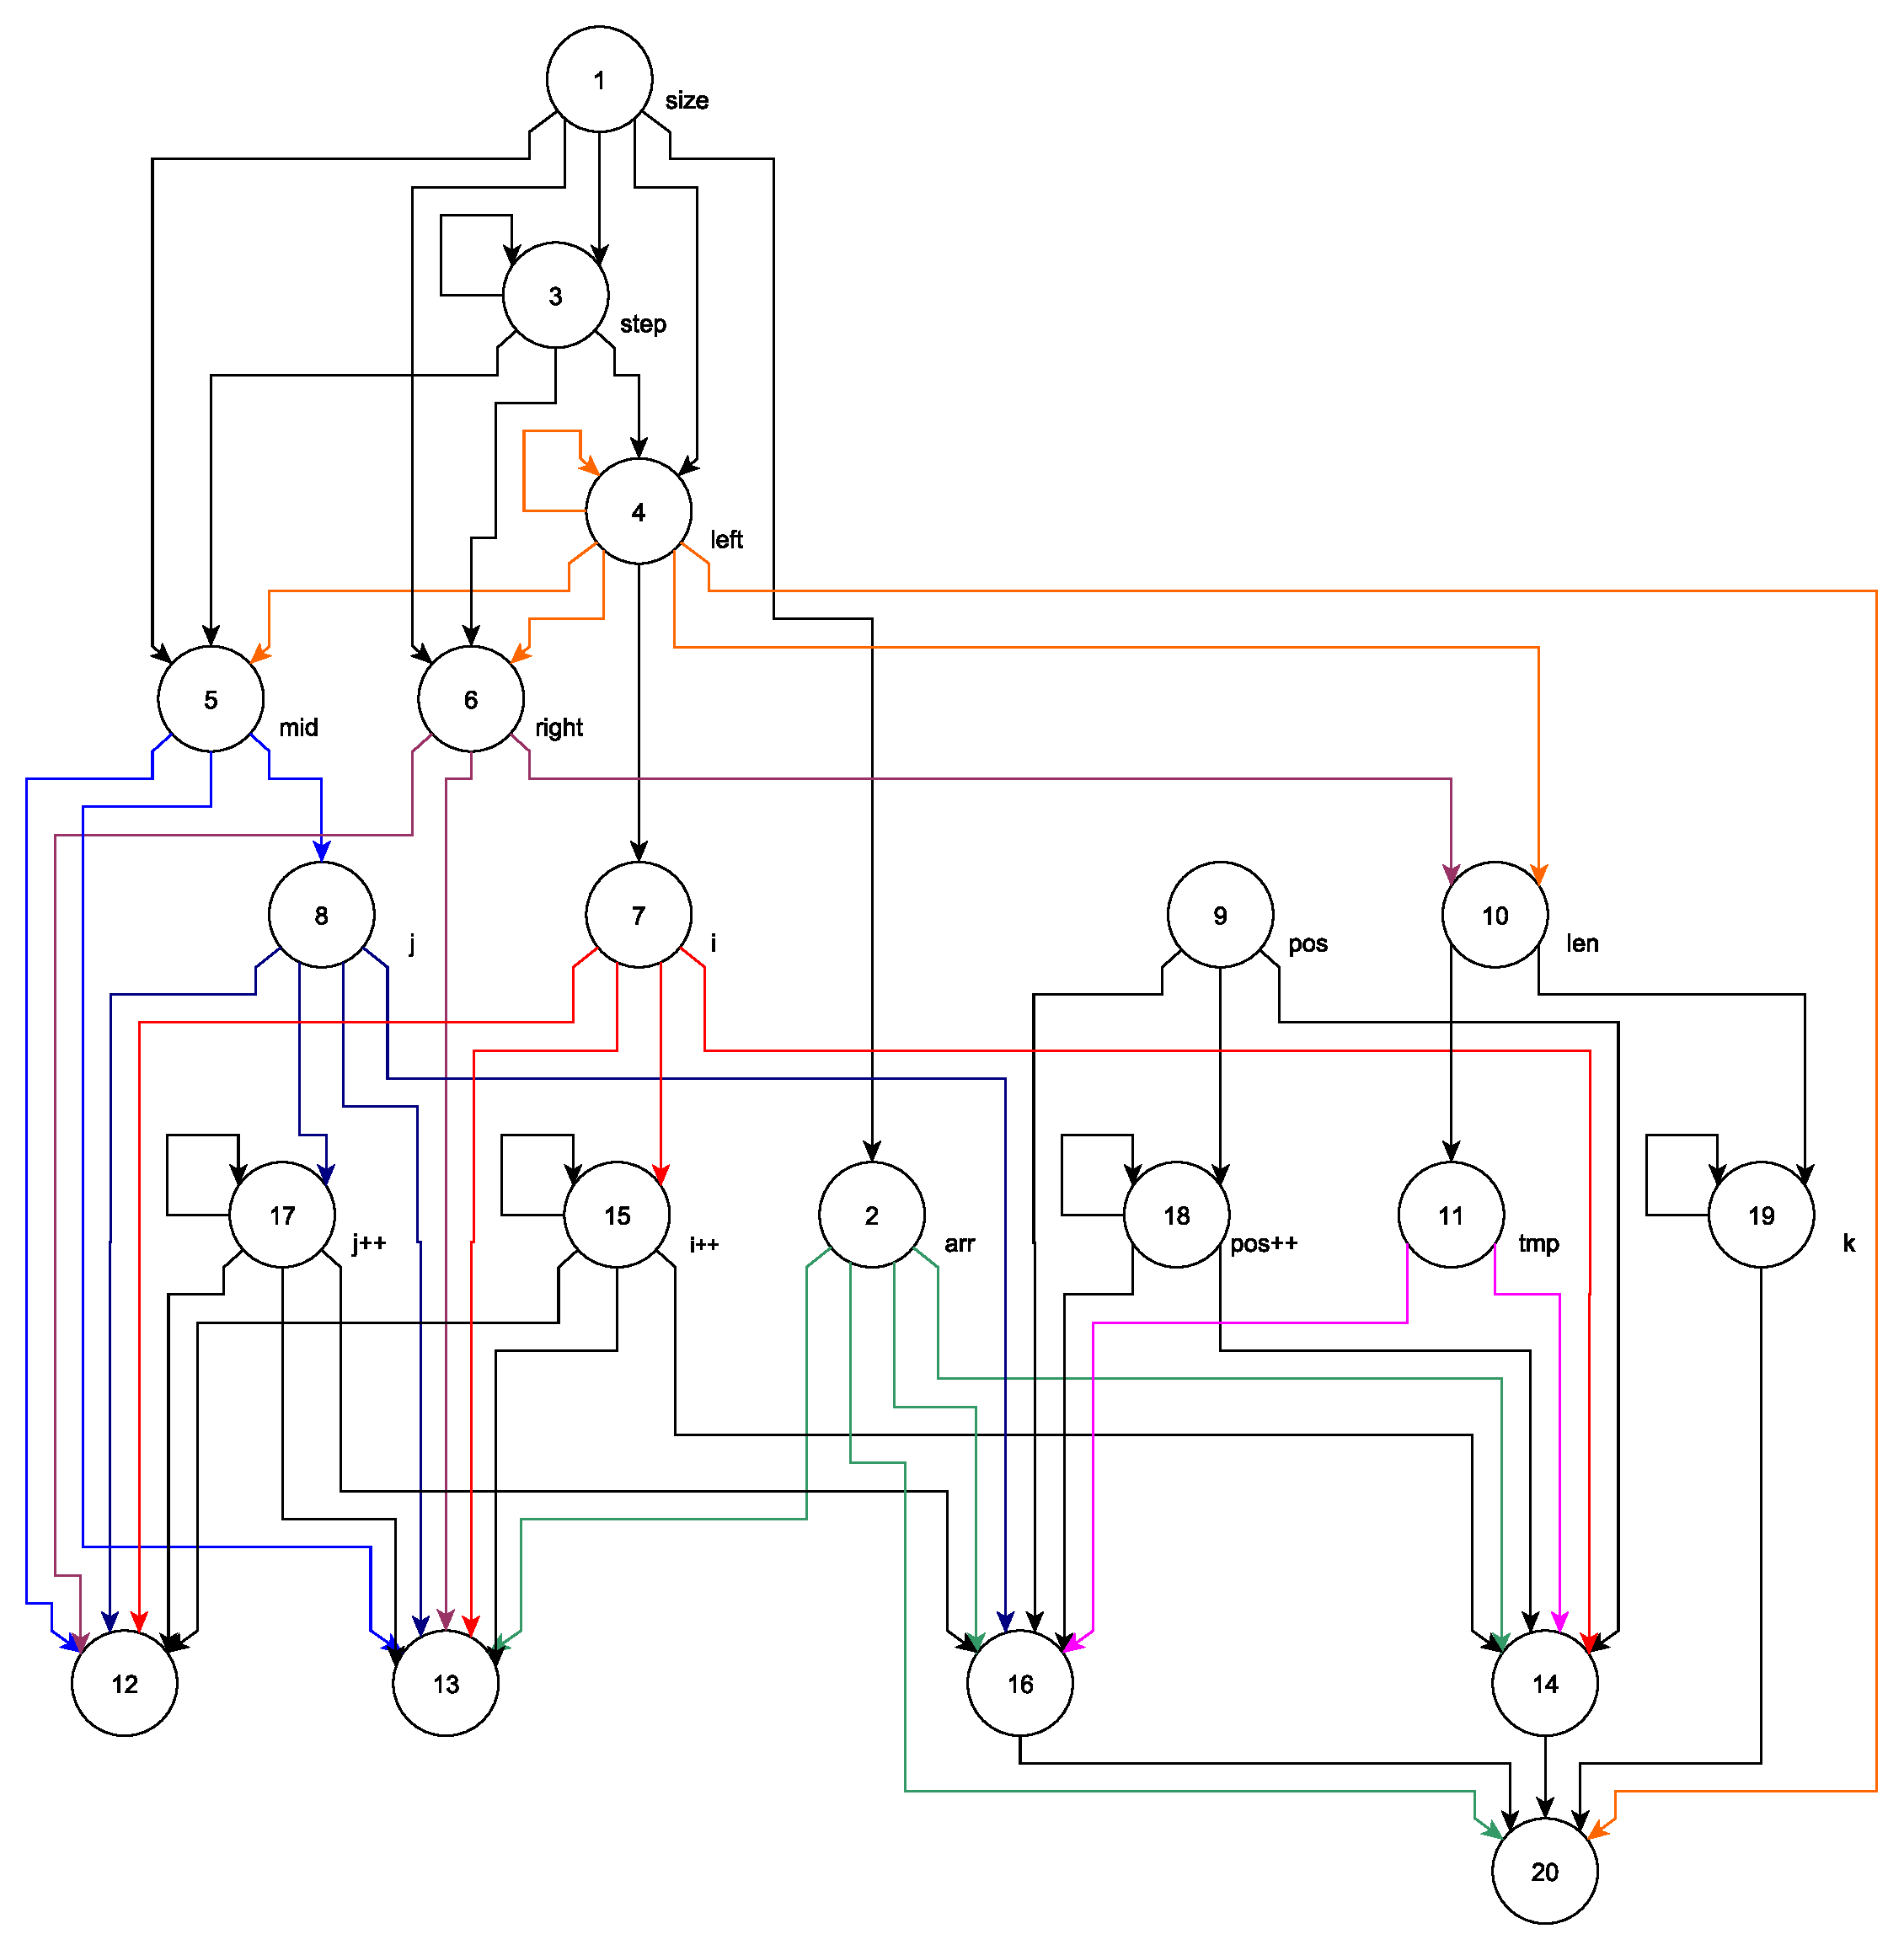
\includegraphics[height=0.6\textheight]{img/информационный_граф.pdf}
	\caption{Информационный граф}
	\label{fg:ig}
\end{figure}

\clearpage

\subsection{Операционная история программы}

Рассмотрим следующий массив: \texttt{a = [4, 3, 2, 1]}.

На рисунках \ref{fg:os_1}--\ref{fg:os_2} представлена операционная история программы для этого массива.

\begin{figure}[h]
	\centering
	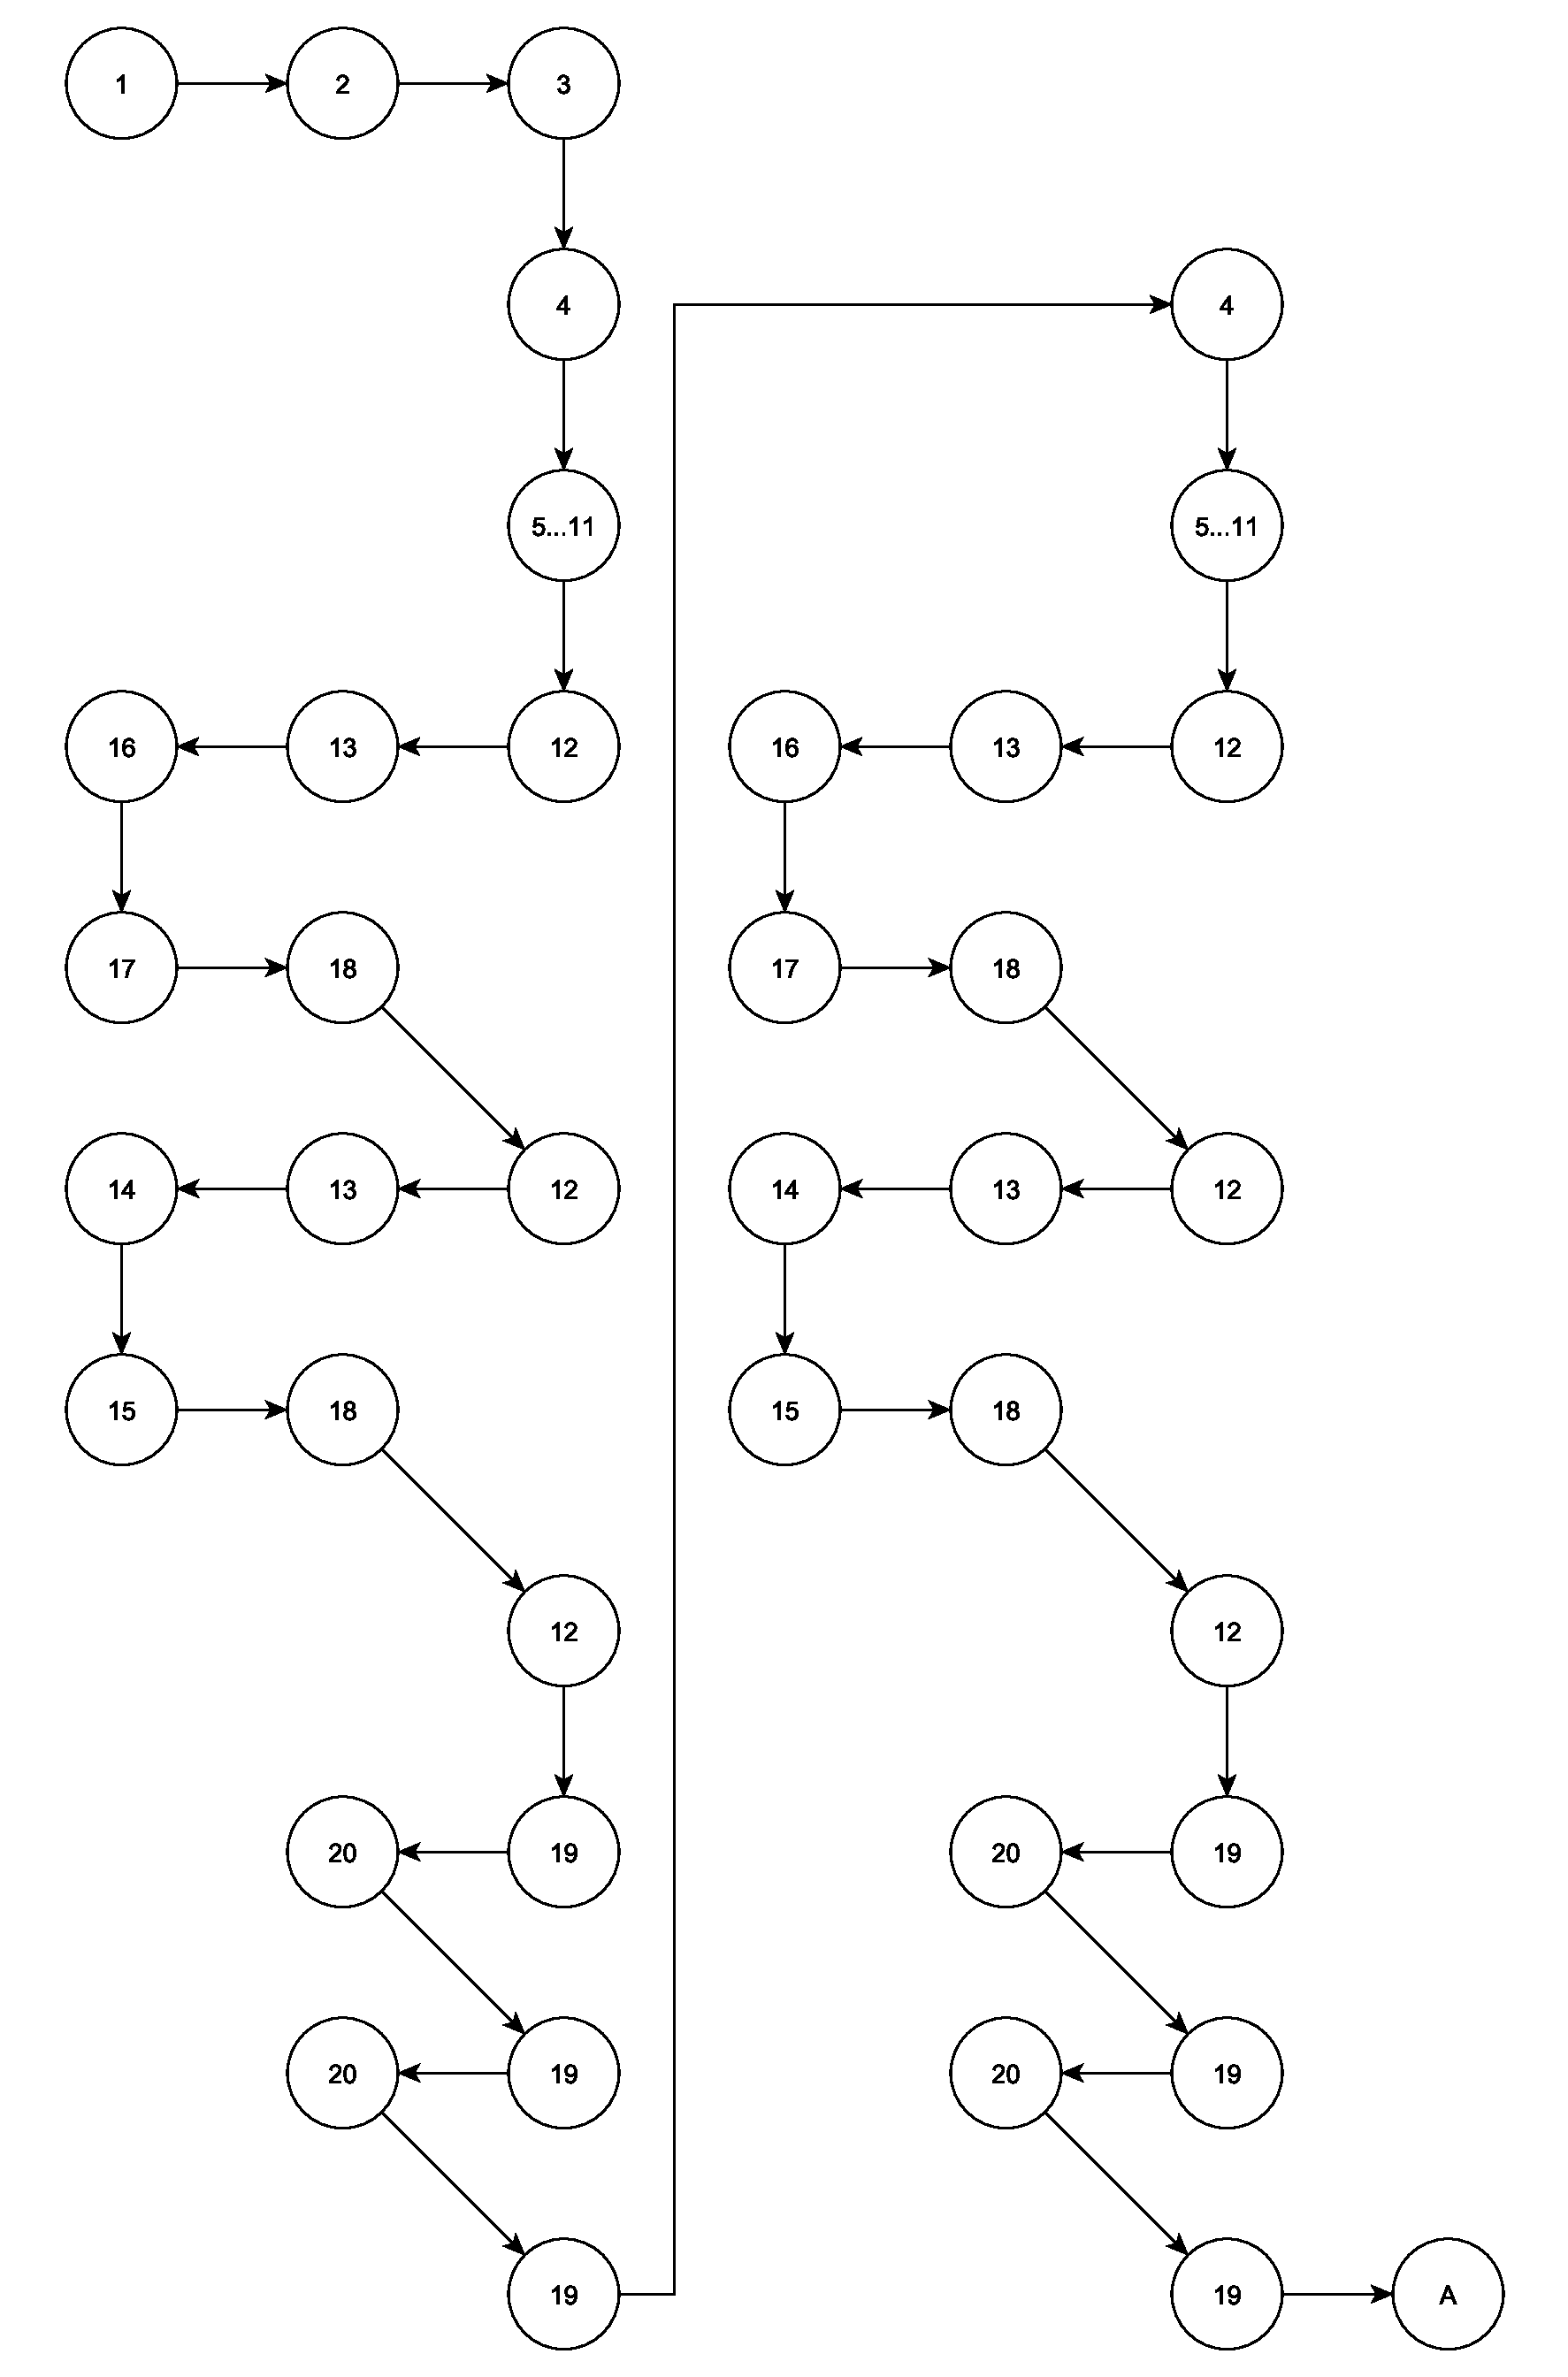
\includegraphics[height=0.7\textheight]{img/операционная_история_1.pdf}
	\caption{Операционная история (начало)}
	\label{fg:oi_1}
\end{figure}

\clearpage

\begin{figure}[h]
	\centering
	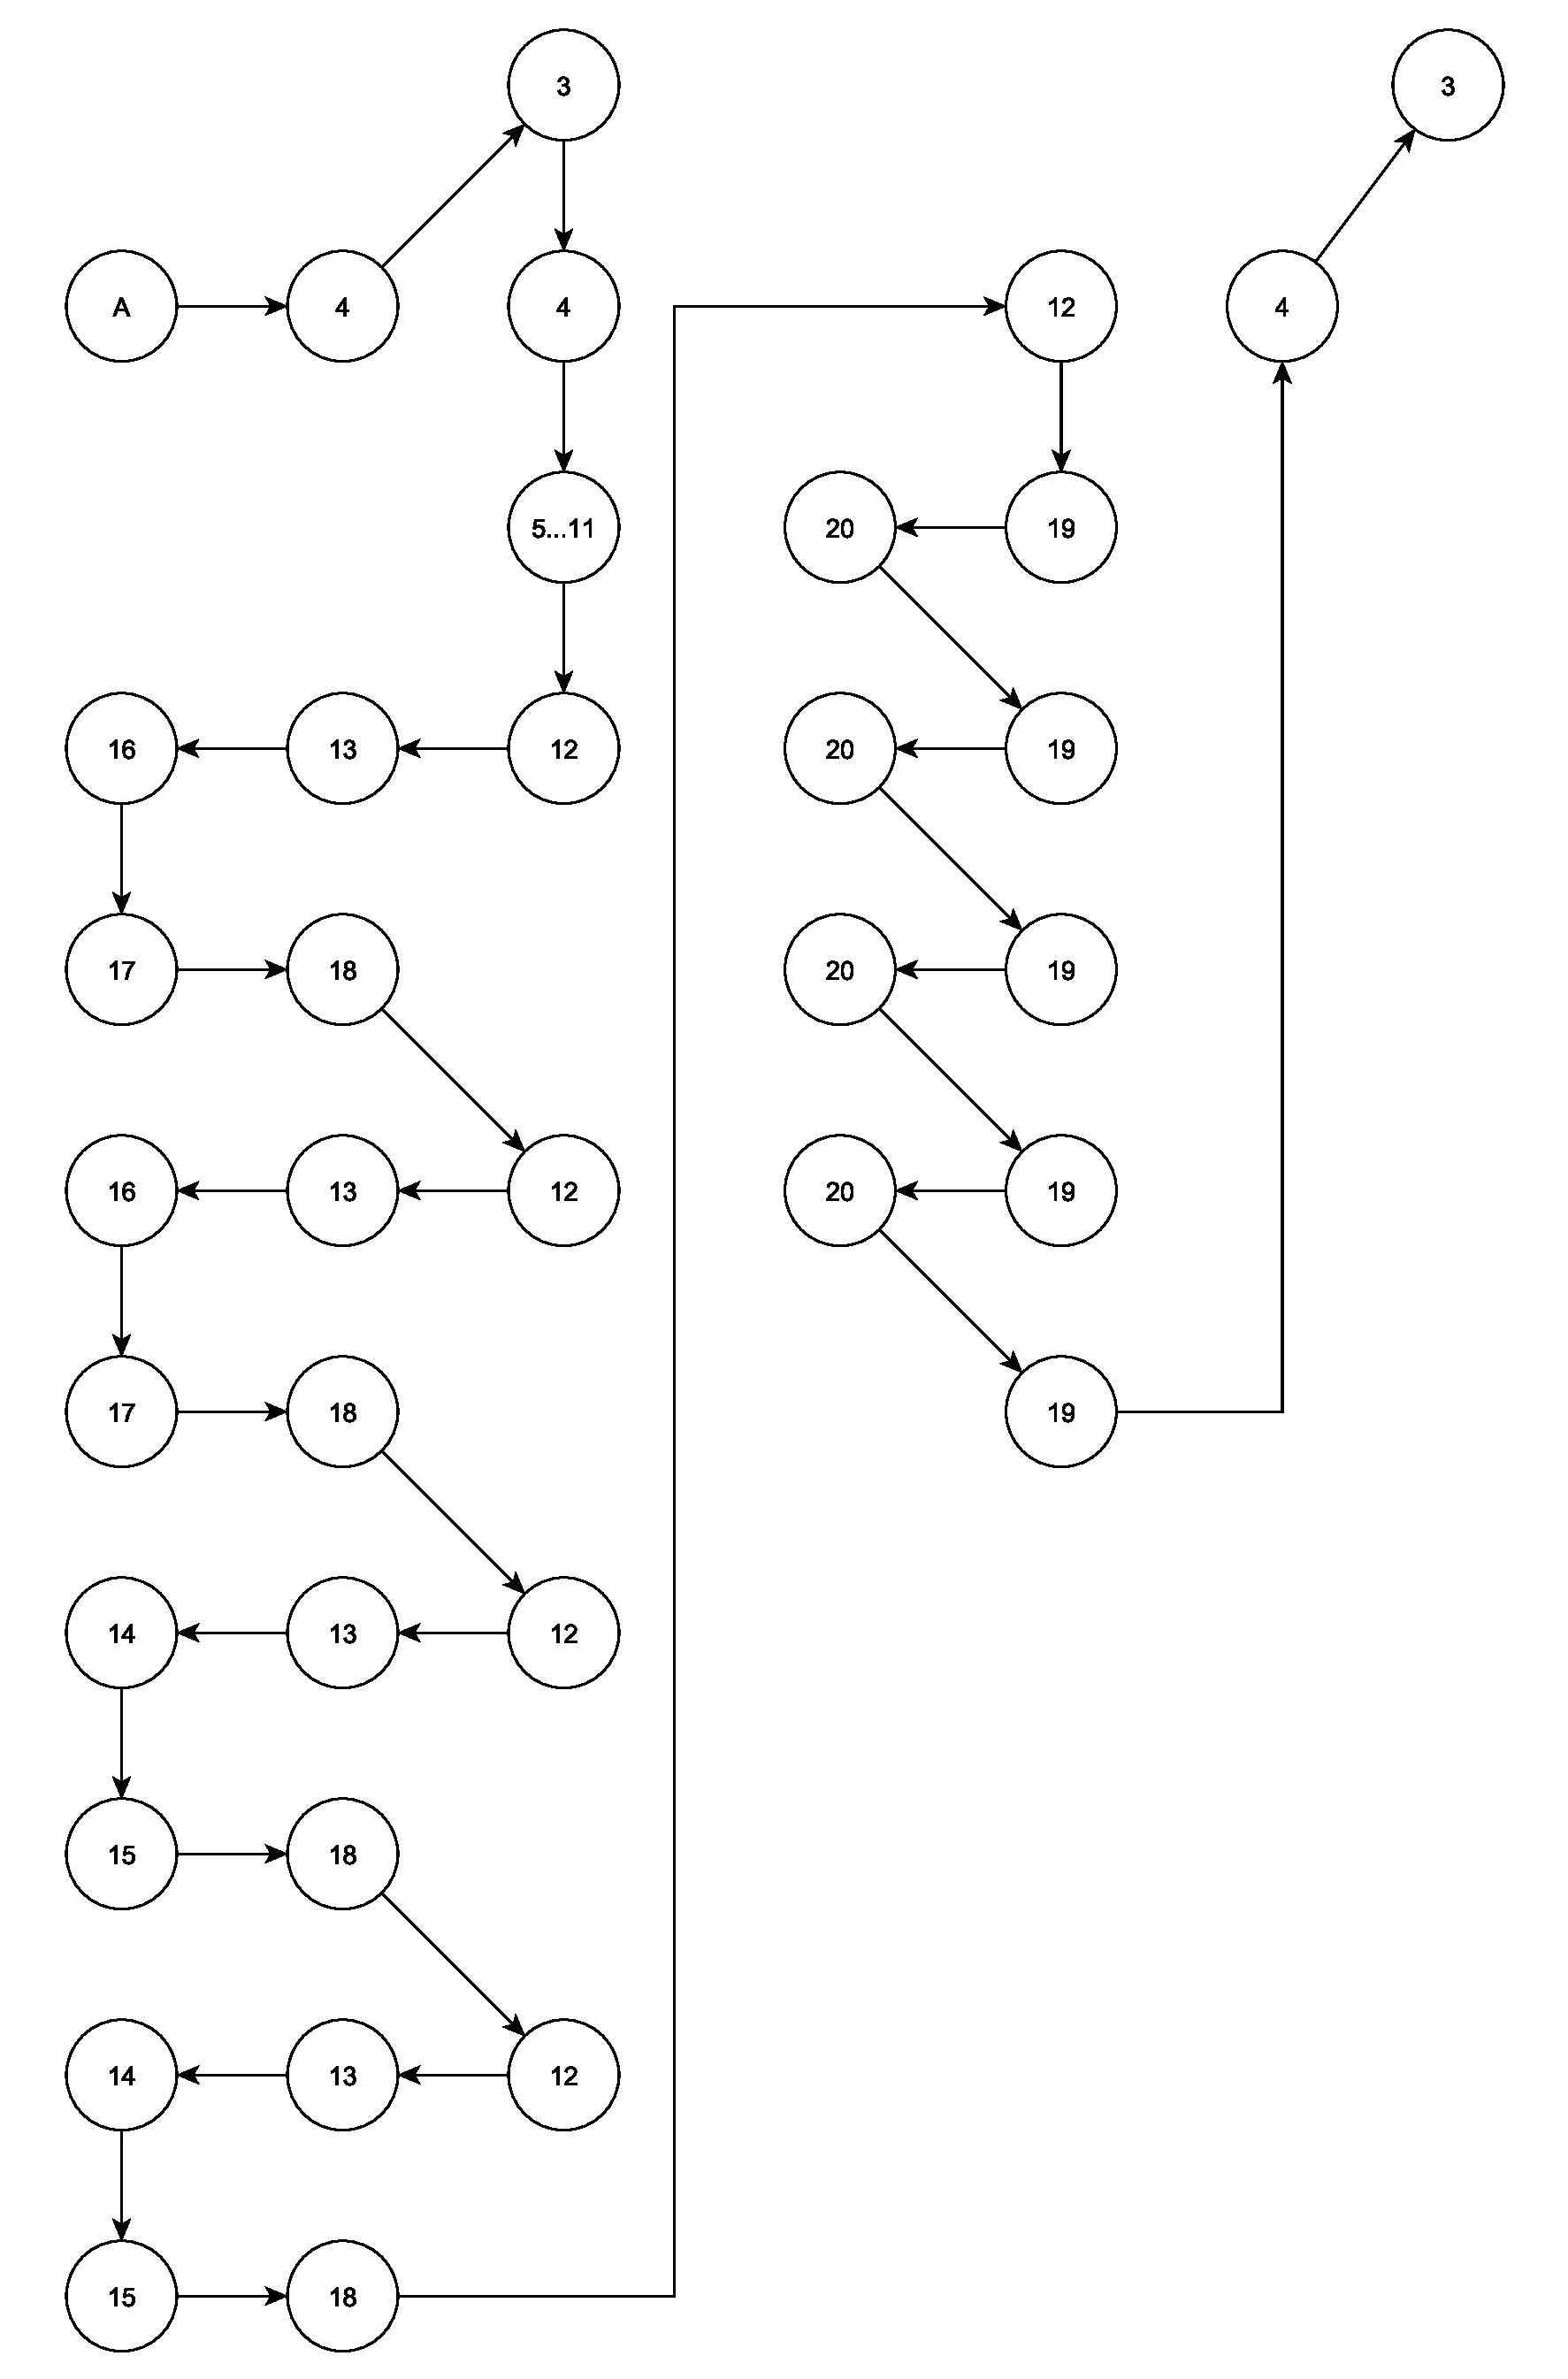
\includegraphics[height=0.9\textheight]{img/операционная_история_2.pdf}
	\caption{Операционная история (конец)}
	\label{fg:oi_2}
\end{figure}

\clearpage

\subsection{Информационная история программы}

\begin{figure}[h]
	\centering
	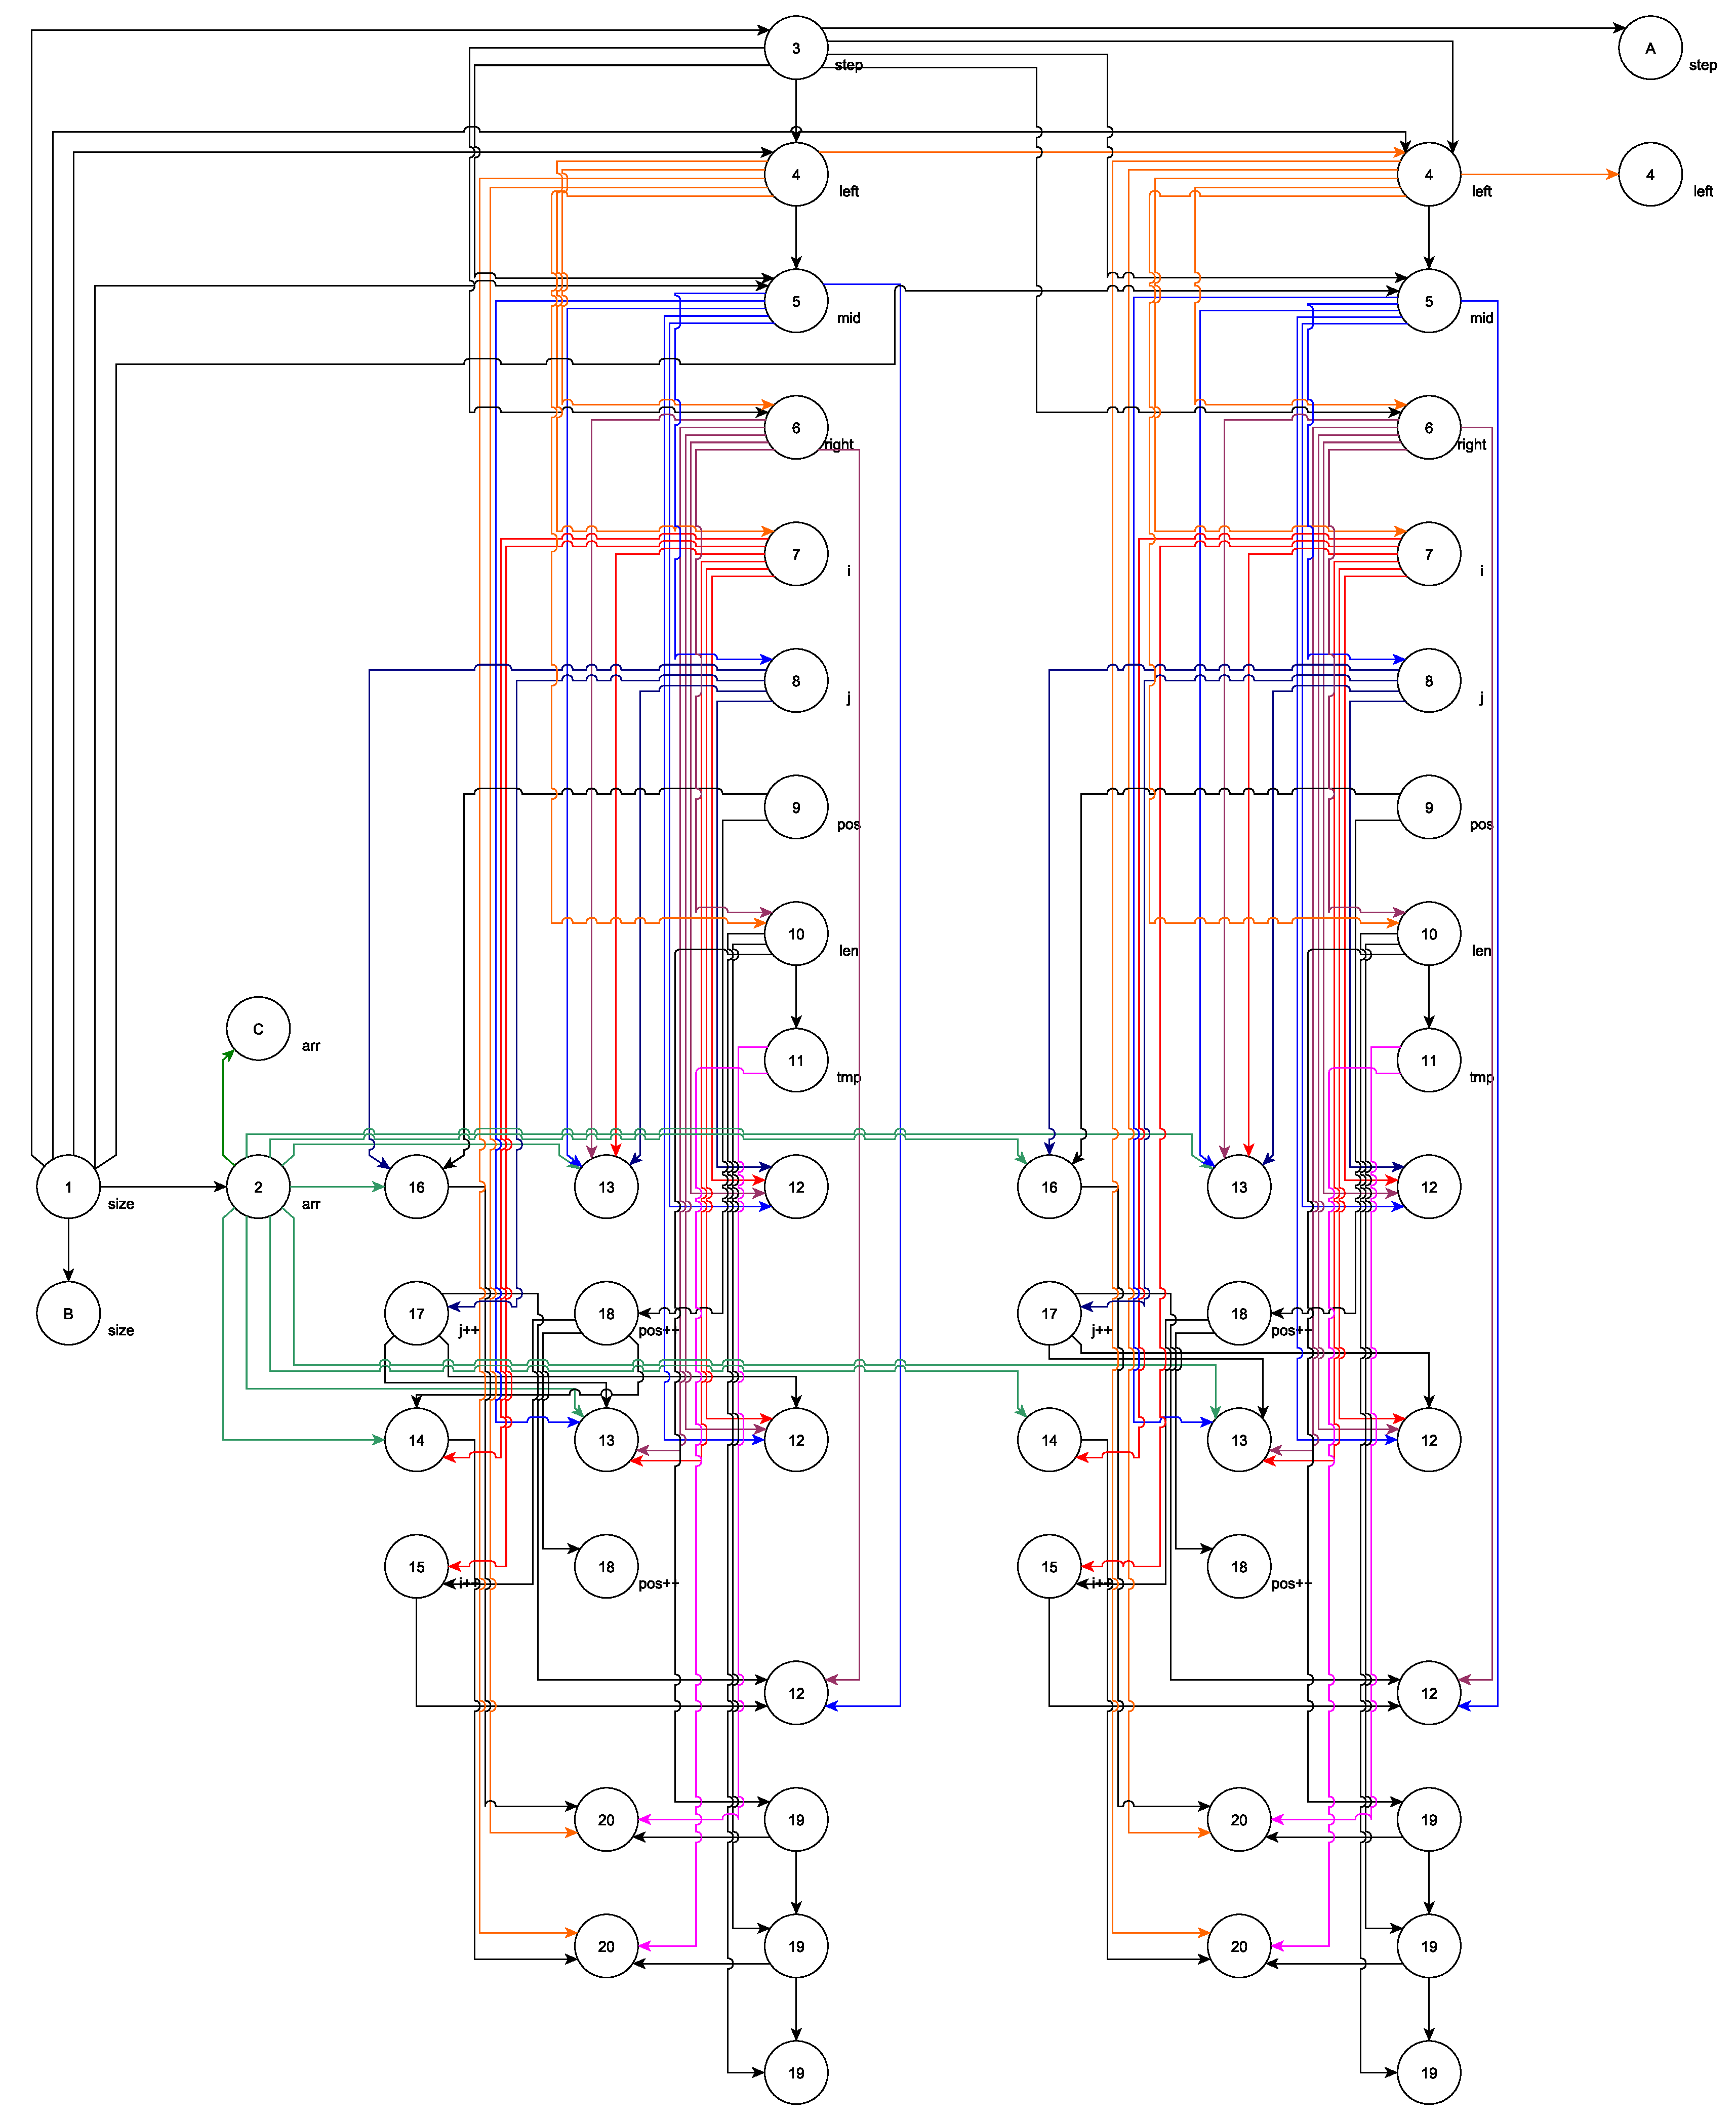
\includegraphics[height=0.7\textheight]{img/информационная_история_1.pdf}
	\caption{Информационная история (начало)}
	\label{fg:ii_1}
\end{figure}

\clearpage

\begin{figure}[h]
	\centering
	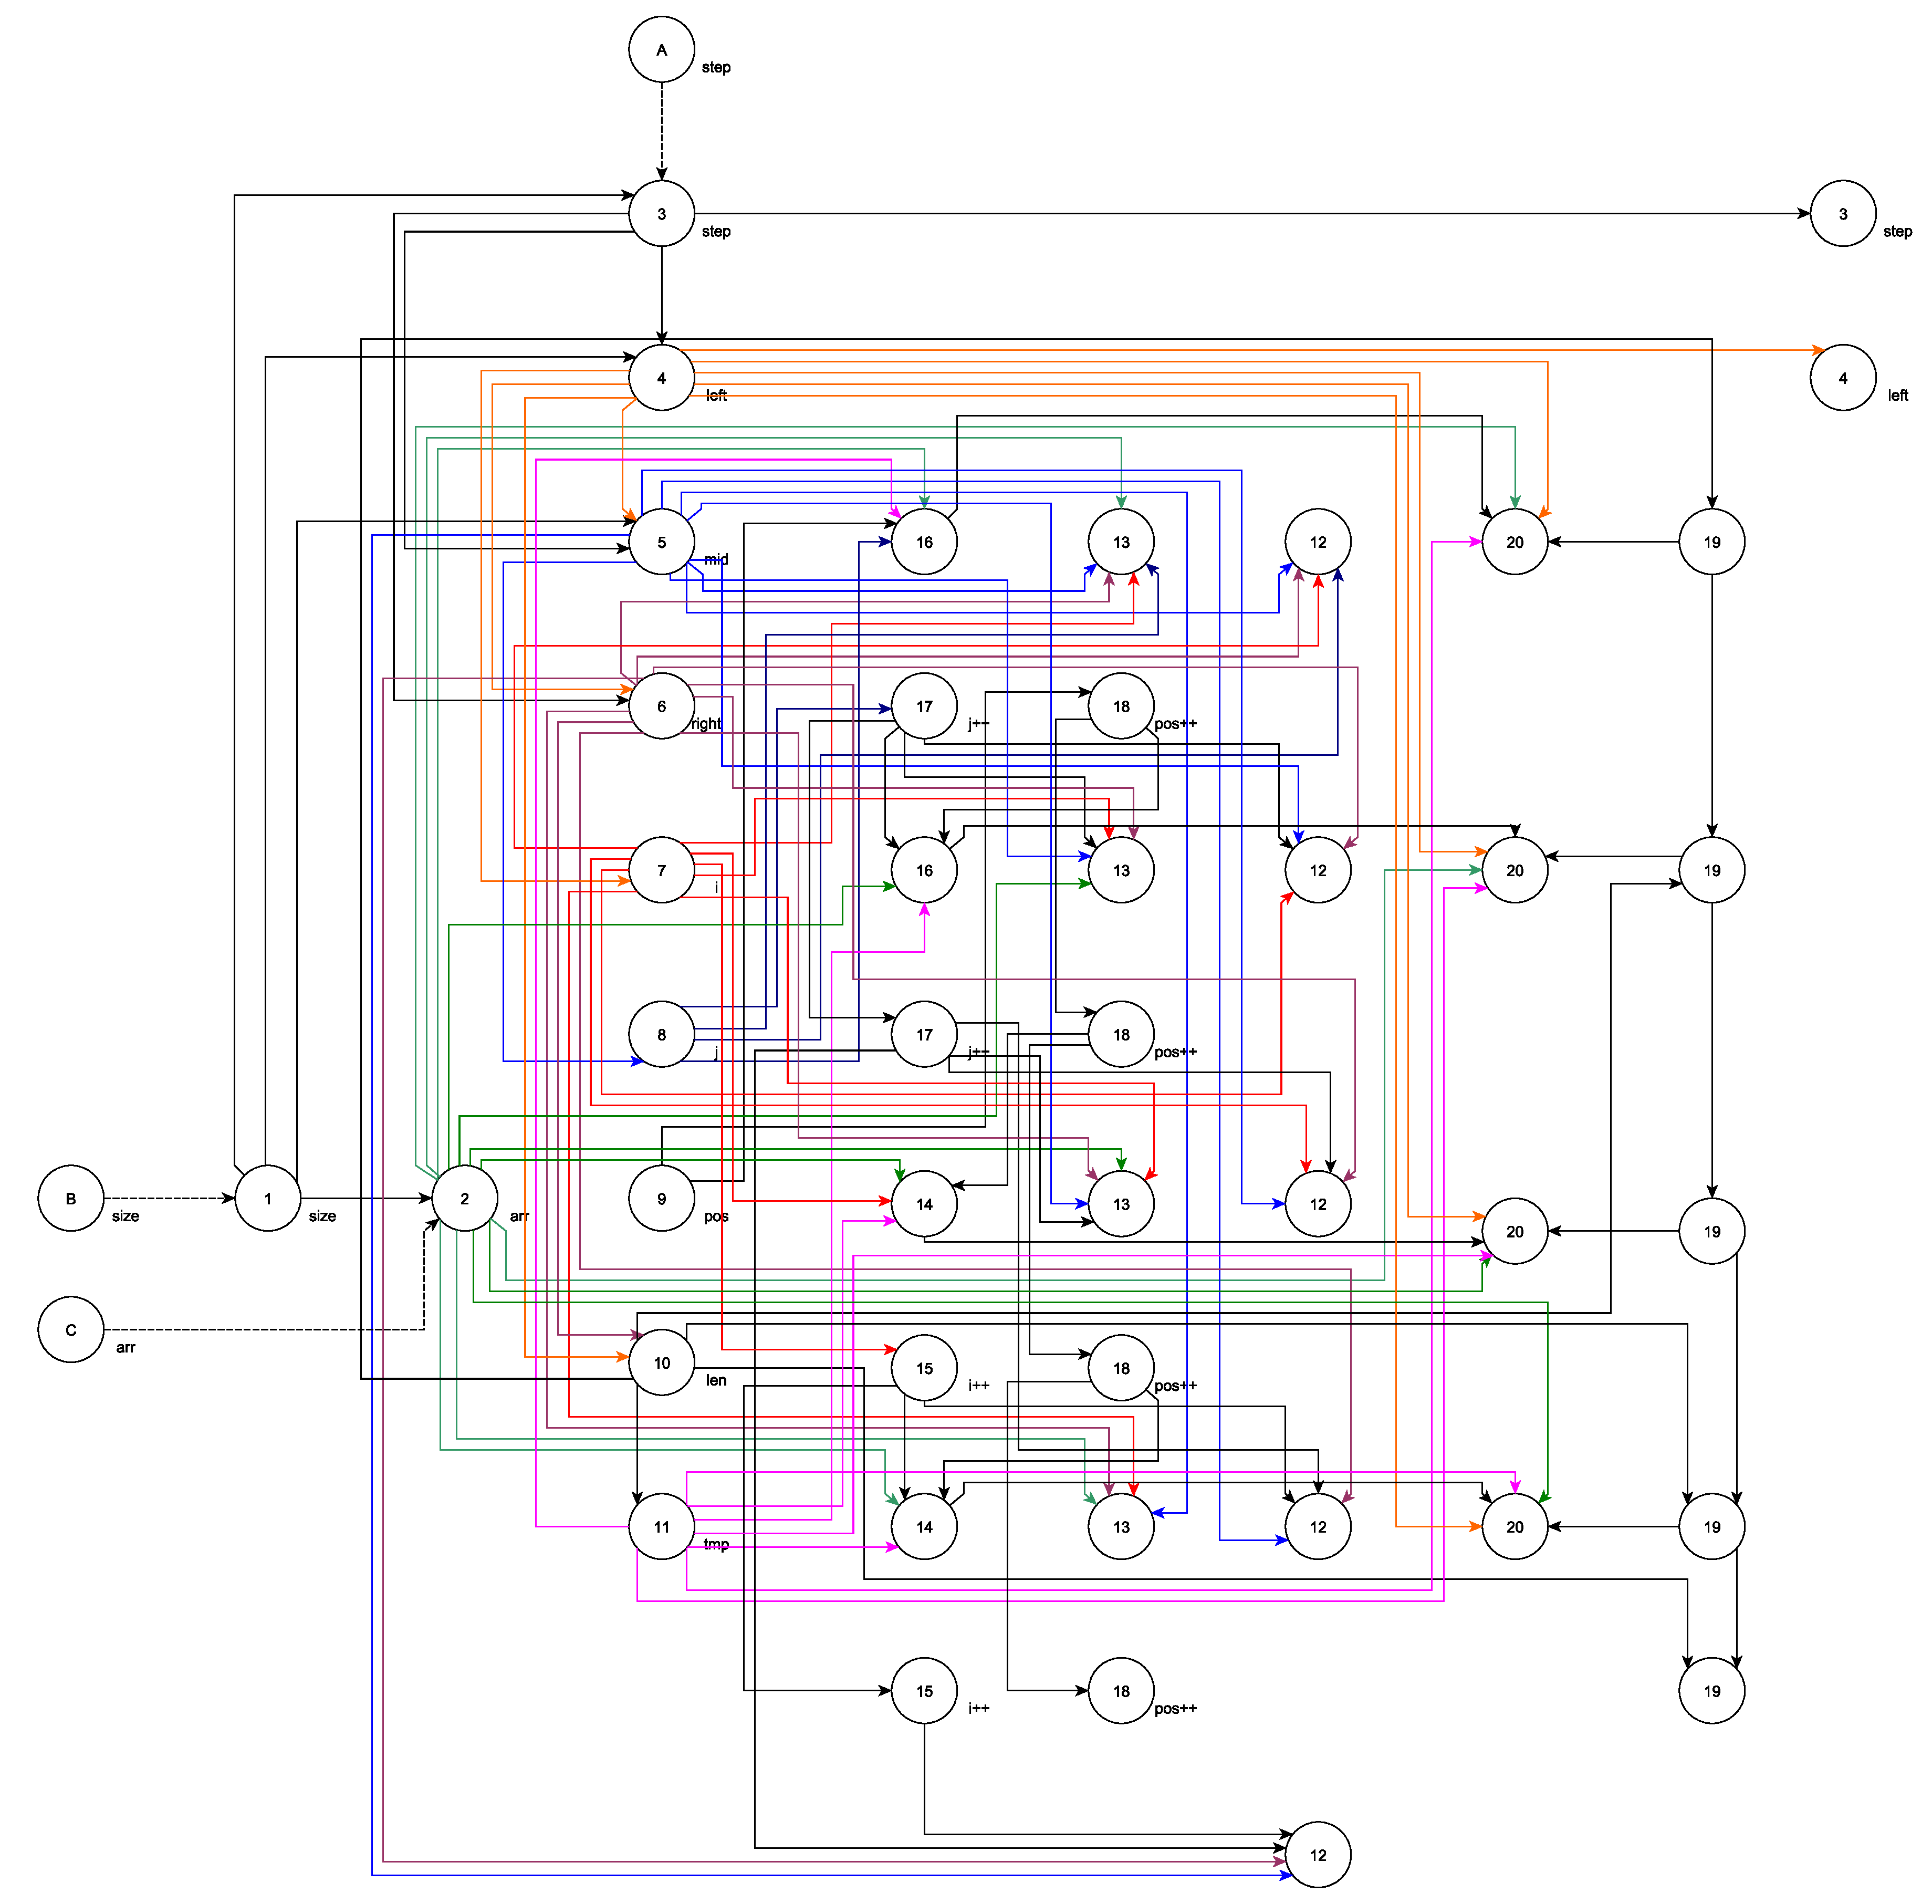
\includegraphics[height=0.6\textheight]{img/информационная_история_2.pdf}
	\caption{Информационная история (конец)}
	\label{fg:ii_2}
\end{figure}

\clearpage

\section*{Возможность распараллеливания}
Можно разделить массив на части и запустить каждую часть сортировки в отдельном потоке, а затем объединить результаты.